\section{Framebuffer 與 Raster Output}

\subsection{Color Buffer 保存與還原}
\label{sec:color-buffer}

程式以 \lstinline|GLUT_SINGLE| 直接繪製在 front buffer。視窗重新出現時系統會要求重畫，但 Scene 往往沒有改變，因此每個 Window 以 \lstinline|ColorBuffer| 保存最後一次完整畫面的 RGBA 像素，並以 contentDirty（內容已改變，需重新 render）與 needsCapture（已 render、尚未擷取）兩個狀態決定重畫方式。如圖~\ref{fig:color-buffer-flow}，display callback 在內容改變、尚未擷取或尺寸不符時重新 render，否則以 \lstinline|glDrawPixels()| 直接還原。擷取則交給每 16 ms 執行一次的 timer，確認內容沒有再次改變後才以 \lstinline|glReadPixels()| 讀回，避免擷取到未完成的畫面。

\begin{figure}[htbp]
    \centering
    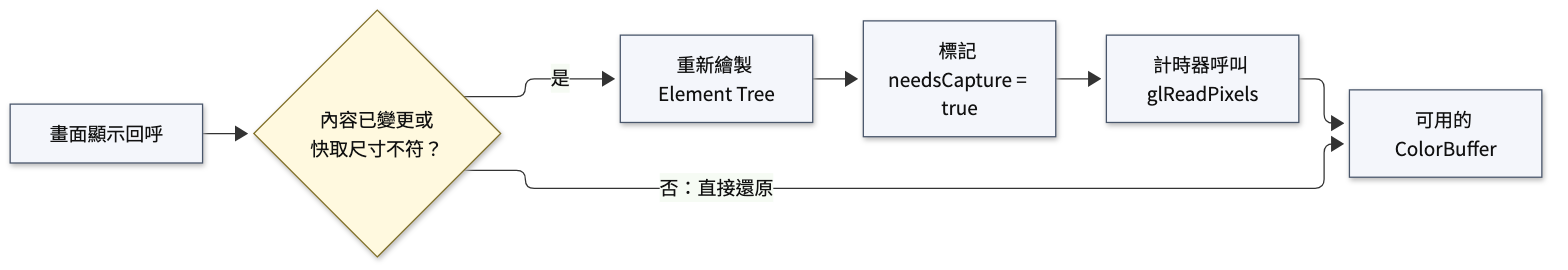
\includegraphics[width=.75\textwidth]{docs/figures/ch06_color-buffer-flow.png}
    \caption{display callback 依內容是否改變，選擇重新 render 或由 ColorBuffer 還原}
    \label{fig:color-buffer-flow}
\end{figure}

修改 Scene 的操作會標記 contentDirty；視窗改變大小時重新配置 ColorBuffer；視窗被隱藏時也會標記 contentDirty，因為 OpenGL 不保證被遮住區域的 front buffer 內容仍然有效。表~\ref{tab:shortcuts} 的 Primary+R 則只要求重畫，會直接還原 ColorBuffer。

\subsection{座標轉換與像素傳輸}
\label{sec:pixel-transfer}

UI 座標以左上角為原點、Y 軸向下，OpenGL 的視窗座標則以左下角為原點、Y 軸向上。對高度為 $H$ 的視窗中左上角為 $(x,y)$、高度為 $h$ 的區域，其 OpenGL 底邊為 $y_{\text{bottom}}=H-y-h$，如圖~\ref{fig:framebuffer-coordinate}。讀回的像素由下往上逐列排列，還原時以相同順序寫回，因此 ColorBuffer 內部不需翻轉；讀寫前也將 pack／unpack alignment 設為 1，使每列像素緊密排列。

\begin{figure}[htbp]
    \centering
    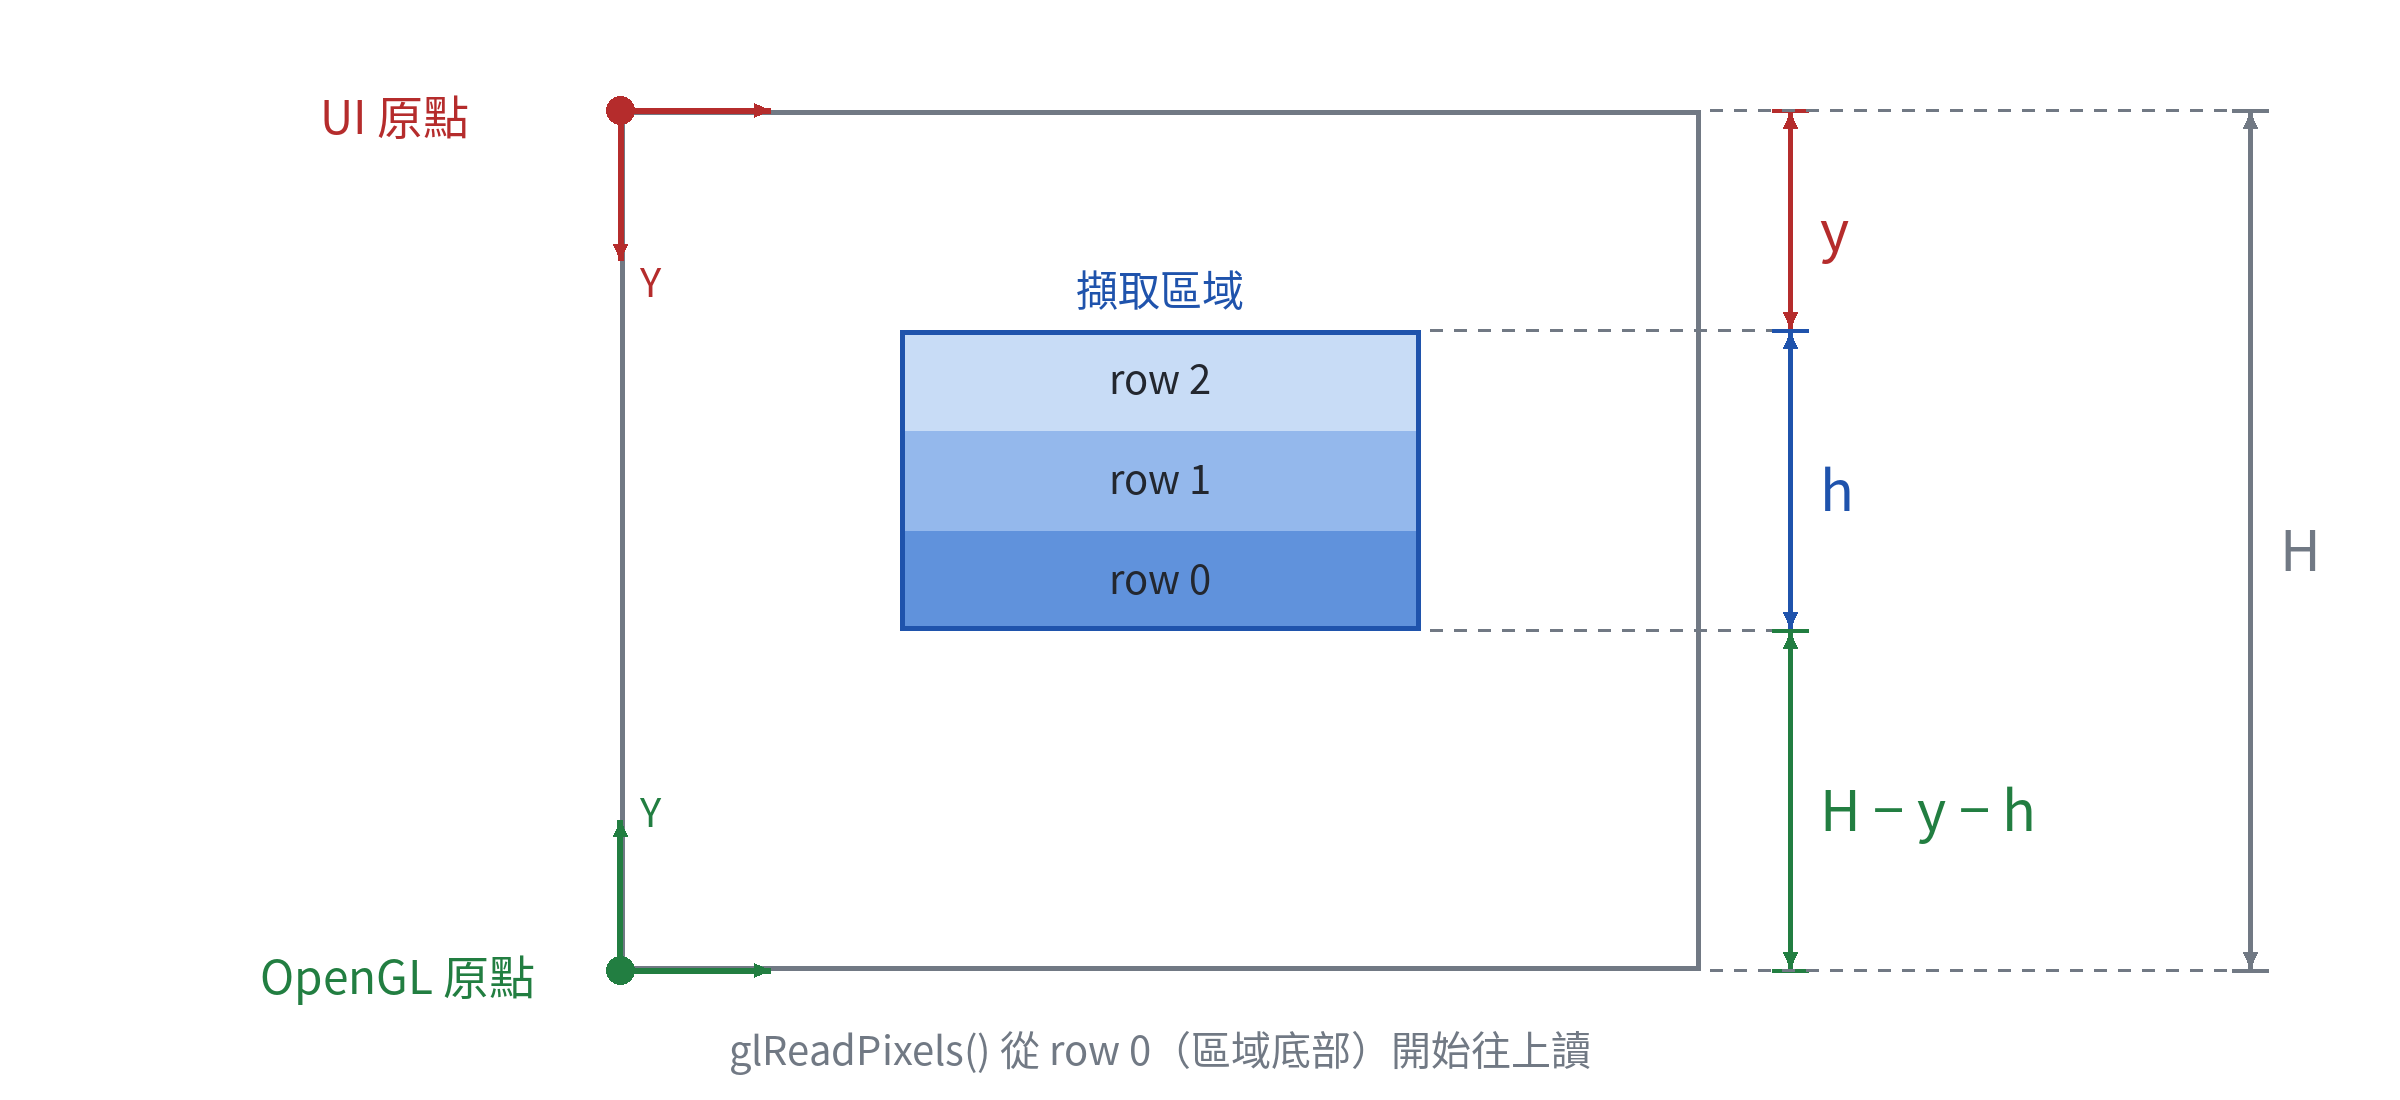
\includegraphics[width=.7\textwidth]{docs/figures/ch06_framebuffer-coordinate.png}
    \caption{同一區域在 UI 座標中由頂端量起（紅），在 OpenGL 中由底端量起（綠）；\lstinline|glReadPixels()| 由區域底部逐列往上讀取}
    \label{fig:framebuffer-coordinate}
\end{figure}

還原時，\lstinline|glRasterPos2f()| 的座標會經過矩陣轉換，不能直接傳入視窗座標。程式先將矩陣設為單位矩陣，以 \lstinline|glRasterPos2f(0, 0)| 將 raster position 設在 viewport 中央，再以不含點陣資料的 \lstinline|glBitmap()| 位移到目標位置，只需 OpenGL 1.1 而不依賴 \lstinline|glWindowPos()|。

\subsection{PPM 圖片輸出}
\label{sec:ppm-export}

主視窗的 ColorBuffer 包含狀態列與 Grid，不能直接輸出。程式另外建立一個與 Canvas 同尺寸、專供匯出使用的視窗，其中只放一個關閉 Grid 的 Canvas，重用相同的 Renderer 繪製 Scene 後擷取。PPM P6 由 header \texttt{P6 $W$ $H$ 255} 與連續的 RGB bytes 組成，像素由頂端逐列往下存放；ColorBuffer 的列順序相反，因此寫檔時從最後一列往前輸出，並捨棄 alpha。實際輸出如圖~\ref{fig:ppm-export}，方向正確且不含 Grid 與狀態列。

\begin{figure}[htbp]
    \centering
    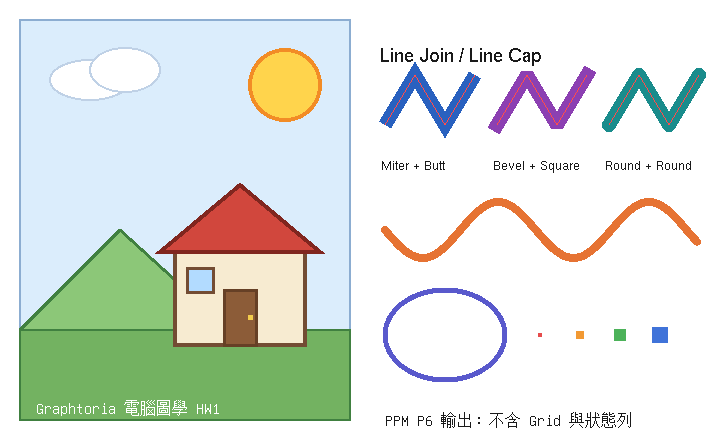
\includegraphics[width=.75\textwidth]{docs/figures/ch07_ppm-showcase.png}
    \caption{程式實際輸出的 PPM P6 圖片（720 × 440，轉為 PNG 後放入報告）}
    \label{fig:ppm-export}
\end{figure}
